% !TEX root = main.tex
\subsection{Relaxationskontrastmessungen}
\label{sec:Signalintensitaet}
Da der zweite Teil des Experiments an einem anderen Versuchstag durchgeführt wurde, wurde zu Beginn erneut eine Optimierung des Aufbaus auf die Wasserprobe vorgenommen um die Vergleichbarkeit der Ergebnisse der beiden Versuchstage zu schaffen. Dies geschah analog zum Vorgehen, welches in Abschnitt \ref{sec:OptimizationandCharacterisationofFIDinwatersample} dargelegt wurde.

Der Versuchsteil selbst zielt darauf ab zu untersuchen, wie longitudinale ($T_1$) und transversale ($T_2$) Relaxationszeit durch paramagnetische Ionen beeinflusst werden können, beziehungsweise welchen Einfluss Veränderungen von $T_1$ und $T_2$ auf die Signalintensität nehmen.
Weiterführend kann dadurch -- abhängig von $T_1$ und $T_2$ -- der Kontrast innerhalb eines bildgebenden Verfahrens verändert werden und somit können verschiedene Bereiche einer Probe besser aufgelöst und analysiert werden. 
Daher sollen die sogenannte Relaxivitäten $r_1$ und $r_2$ nach
\begin{align}
    \frac{1}{T_{\text{i}}\left([\ce{X^2+}]\right)} = r_{\text{i}} \cdot [\ce{X^2+}] + \frac{1}{T_{\text{i}}(0)} \label{eq:relaxivitat}
\end{align}
bestimmt werden. Dabei bezeichnet $T_{\text{i}}\left([\ce{X^2+}]\right)$ die -- von der Konzentration des verwendeten paramagnetischen Salzes im Wasser abhängige -- jeweilige Relaxationszeit, $[\ce{X^2+}]$  die entsprechende Ionenkonzentration des jeweiligen Stoffs und $T_{\text{i}}(0)$ die Relaxationszeit im Falle, dass kein Kontrastmittel verwendet wird.\newline
Bei bildgebenden Verfahren auf Grundlage der Magnetresonanz können in erster Linie Bereiche unterschiedlicher Spindichte graphisch aufgelöst und analysiert werden.
Sollte es von Interesse sein Bereiche gleicher Spindichte kontrastreich abzubilden, so sind weiterführende Methoden von Nöten.
Eine Methode ist dabei das Verwenden von Kontrastmitteln um die Relaxationszeiten zu beeinflussen und damit die Signalintensität zu verändern.
Es wird von positivem Kontrast gesprochen, sofern die Signalintensität erhöht werden kann, respektive von negativem bei Verringerung der Intensität. 
Die Signalintensität kann dadurch erhöht werden, dass die longitudinale Relaxationszeit verringert wird.
Dies führt dazu, dass sich die Spins während des polarisierenden Pulses schneller entlang des angelegten B-Feldes orientieren.
Eine geringe Intensität erreichtman beispielsweise durch das verringern der transversalen Relaxationszeit.
Dann relaxieren die Spins entsprechend schneller in der transversalen Ebene und die Signalintensität verringert sich entsprechend zügig.
Im vorliegenden Versuch wurden paramagnetische Kontrastmittel in Form von in einer Wasserprobe (\SI{500}{\milli \liter}) gelöstem Kupfer- (\ce{Cu^2+}) und Mangansalz (\ce{Mn^2+}) eingesetzt.
Zudem wurden unterschiedliche Konzentrationen der Kontrastmittel untersucht. 
Für das zweifach positiv geladene Kupfer lagen die verwendeten Stoffmengen bei \SI{250}{\micro \mol}, \SI{500}{\micro \mol}, \SI{1000}{\micro \mol} und \SI{2000}{\micro \mol}, bei Mangan waren dies Werte von \SI{25}{\micro \mol}, \SI{50}{\micro \mol}, \SI{100}{\micro \mol} und \SI{200}{\micro \mol}.
Die Besonderheit paramagnetischer Kontrastmittel liegt im Vorliegen ungepaarter Elektronen und der positiven magnetischen Suszeptibilität.
Letztere beeinflusst die longitudinale Relaxationszeit $T_1$ dadurch, dass lokal ein magnetisches Feld generiert wird bzw. das von außen angelegte B-Feld unterstützt wird, dadruch orientieren sich die Spins schneller entlang des Magnetfeldes.
Somit wird $T_1$ verringert.
Gleiches gilt auch für $T_2$ allerdings spielen hierbei auch die ungepaarten Elektronen eine Rolle, welche die Spin-Spin-Wechselwirkungen verstärken und somit $T_2$ zusätzlich verringern.
Wie oben bereits beschrieben bewirkt eine Verringerung von $T_1$ einen positiven Kontrast, die Verringerung von $T_2$ hingegen einen negativen.
Bei geringer Konzentration der Kontrastmittel wird $T_1$ stärker beeinflusst da der Einfluss der positiven magnetischen Suszeptibilität schon bei geringer Stoffmenge deutlich zu erkennen ist.
Im Gegensatz dazu ist der Effekt durch zusätzliche ungepaarte Elektronen erst bei hohen Konzentrationen der Kontratsmittel deutlich in den Messungen der transversalen Relaxationszeit zu verzeichnen. \cite{Schmidt}

\begin{figure}[H]
    \centering
    % !TEX root = main.tex
\section{Fourietrafo der Messungen mit unterschieldicheer Polarisationszeit}
\begin{figure}[H]
    \centering
    % !TEX root = main.tex
\section{Fourietrafo der Messungen mit unterschieldicheer Polarisationszeit}
\begin{figure}[H]
    \centering
    % !TEX root = main.tex
\section{Fourietrafo der Messungen mit unterschieldicheer Polarisationszeit}
\begin{figure}[H]
    \centering
    \input{plots/Polarisationszeit.tex}
    \caption{Amplitude in abhängigkeit von zwei verschiedenen Piolarisatiosnzeiten}
\end{figure}
    \caption{Amplitude in abhängigkeit von zwei verschiedenen Piolarisatiosnzeiten}
\end{figure}
    \caption{Amplitude in abhängigkeit von zwei verschiedenen Piolarisatiosnzeiten}
\end{figure}
    \caption[Abhängigkeit der Signalintensität von der Polarisationszeit.]{In dieser Abbildung sind zwei ,,Pulse and Collect''-Messungen der bidestillierten Wasserprobe dargestellt. Die rote Kurve zeigt eine Messung mit einer Polarisationszeit von $\SI{4}{\second}$, bei der blauen Kurve beträgt die Polarisationszeit $\SI{0.5}{\second}$. Hierbei ist deutlich zu erkennen, dass die Signalintensität durch die höhere Polarisationszeit deutlich gesteigert werden kann. Bei den dargestellten Messungen um circa Faktor drei.} 
    \label{fig:SignalintensitaetPolarisationszeit}    
\end{figure}

Am Versuchstag wurden zunächst zwei ,,Pulse and Collect''-Messungen einer Wasserprobe mit unterschiedlicher Polarisationszeit vorgenommen.
Abbildung \ref{fig:SignalintensitaetPolarisationszeit} zeigt die entsprechenden Kurven.
Dabei ist zu erkennen, dass bei geringerer Polarisationszeit (\SI{0.5}{\second}) eine deutlich geringere Amplitude bzw. Signalintensität vorliegt.
Dies war nach den Erkenntnissen des ersten Abschnitts \ref{sec:PartI} auch so erwartbar.
Unter Verwendung einer, mit einem unbekannten paramagnetischen Stoff versetzten, Wasserprobe hätte nun der Einfluss dieses Stoffs auf $T_1$ und damit die Signalintensität untersucht werden sollen.
Es wäre zu erwarten gewesen, dass sich auch bei kürzerer Polarisationszeit in diesem Fall kein deutlicher Abfall der Signalintensität ergibt.
Dies ist wie oben angedeutet damit zu begründen, dass die longitudinale Relaxationszeit kleiner wird und somit schon eine kürzere Polarisationszeit genügt um alle Spins gleichzurichten und somit ein gutes Signal zu erhalten.
Allerdings wurden die entsprechenden Messreihen am Versuchstag zwar durchgeführt und entsprechende Resultate erkannt, jedoch wurden dies aus unbekannten Gründen nicht abgespeichert und können somit an dieser Stelle nicht präsentiert werden.\newline
\newline
Im nächsten Schritt wurden dann die longitudinale und transversale Relaxationszeit der Wasserprobe ermittelt.
Die Vorgehensweisen entsprachen dabei den in den Kapiteln \ref{sec:LongitudinalrelaxationmeasurementsT1} und \ref{sec:Transversalrelaxationmeasurements} diskutieren Verfahren.
Die entsprechenden Messreihen sind in Abbildung \ref{fig:T1T2Wasser} dargestellt.

\begin{figure}[H]
    \begin{subfigure}[b]{0.5\textwidth}
        \centering
        \resizebox{1\textwidth}{!}{% GNUPLOT: LaTeX picture with Postscript
\begingroup
  % Encoding inside the plot.  In the header of your document, this encoding
  % should to defined, e.g., by using
  % \usepackage[cp1252,<other encodings>]{inputenc}
  \inputencoding{cp1252}%
  \makeatletter
  \providecommand\color[2][]{%
    \GenericError{(gnuplot) \space\space\space\@spaces}{%
      Package color not loaded in conjunction with
      terminal option `colourtext'%
    }{See the gnuplot documentation for explanation.%
    }{Either use 'blacktext' in gnuplot or load the package
      color.sty in LaTeX.}%
    \renewcommand\color[2][]{}%
  }%
  \providecommand\includegraphics[2][]{%
    \GenericError{(gnuplot) \space\space\space\@spaces}{%
      Package graphicx or graphics not loaded%
    }{See the gnuplot documentation for explanation.%
    }{The gnuplot epslatex terminal needs graphicx.sty or graphics.sty.}%
    \renewcommand\includegraphics[2][]{}%
  }%
  \providecommand\rotatebox[2]{#2}%
  \@ifundefined{ifGPcolor}{%
    \newif\ifGPcolor
    \GPcolorfalse
  }{}%
  \@ifundefined{ifGPblacktext}{%
    \newif\ifGPblacktext
    \GPblacktexttrue
  }{}%
  % define a \g@addto@macro without @ in the name:
  \let\gplgaddtomacro\g@addto@macro
  % define empty templates for all commands taking text:
  \gdef\gplbacktext{}%
  \gdef\gplfronttext{}%
  \makeatother
  \ifGPblacktext
    % no textcolor at all
    \def\colorrgb#1{}%
    \def\colorgray#1{}%
  \else
    % gray or color?
    \ifGPcolor
      \def\colorrgb#1{\color[rgb]{#1}}%
      \def\colorgray#1{\color[gray]{#1}}%
      \expandafter\def\csname LTw\endcsname{\color{white}}%
      \expandafter\def\csname LTb\endcsname{\color{black}}%
      \expandafter\def\csname LTa\endcsname{\color{black}}%
      \expandafter\def\csname LT0\endcsname{\color[rgb]{1,0,0}}%
      \expandafter\def\csname LT1\endcsname{\color[rgb]{0,1,0}}%
      \expandafter\def\csname LT2\endcsname{\color[rgb]{0,0,1}}%
      \expandafter\def\csname LT3\endcsname{\color[rgb]{1,0,1}}%
      \expandafter\def\csname LT4\endcsname{\color[rgb]{0,1,1}}%
      \expandafter\def\csname LT5\endcsname{\color[rgb]{1,1,0}}%
      \expandafter\def\csname LT6\endcsname{\color[rgb]{0,0,0}}%
      \expandafter\def\csname LT7\endcsname{\color[rgb]{1,0.3,0}}%
      \expandafter\def\csname LT8\endcsname{\color[rgb]{0.5,0.5,0.5}}%
    \else
      % gray
      \def\colorrgb#1{\color{black}}%
      \def\colorgray#1{\color[gray]{#1}}%
      \expandafter\def\csname LTw\endcsname{\color{white}}%
      \expandafter\def\csname LTb\endcsname{\color{black}}%
      \expandafter\def\csname LTa\endcsname{\color{black}}%
      \expandafter\def\csname LT0\endcsname{\color{black}}%
      \expandafter\def\csname LT1\endcsname{\color{black}}%
      \expandafter\def\csname LT2\endcsname{\color{black}}%
      \expandafter\def\csname LT3\endcsname{\color{black}}%
      \expandafter\def\csname LT4\endcsname{\color{black}}%
      \expandafter\def\csname LT5\endcsname{\color{black}}%
      \expandafter\def\csname LT6\endcsname{\color{black}}%
      \expandafter\def\csname LT7\endcsname{\color{black}}%
      \expandafter\def\csname LT8\endcsname{\color{black}}%
    \fi
  \fi
    \setlength{\unitlength}{0.0500bp}%
    \ifx\gptboxheight\undefined%
      \newlength{\gptboxheight}%
      \newlength{\gptboxwidth}%
      \newsavebox{\gptboxtext}%
    \fi%
    \setlength{\fboxrule}{0.5pt}%
    \setlength{\fboxsep}{1pt}%
\begin{picture}(7200.00,5040.00)%
    \gplgaddtomacro\gplbacktext{%
      \csname LTb\endcsname%%
      \put(814,704){\makebox(0,0)[r]{\strut{}$0$}}%
      \put(814,1527){\makebox(0,0)[r]{\strut{}$0.2$}}%
      \put(814,2350){\makebox(0,0)[r]{\strut{}$0.4$}}%
      \put(814,3173){\makebox(0,0)[r]{\strut{}$0.6$}}%
      \put(814,3996){\makebox(0,0)[r]{\strut{}$0.8$}}%
      \put(814,4819){\makebox(0,0)[r]{\strut{}$1$}}%
      \put(946,484){\makebox(0,0){\strut{}$0$}}%
      \put(1660,484){\makebox(0,0){\strut{}$500$}}%
      \put(2375,484){\makebox(0,0){\strut{}$1000$}}%
      \put(3089,484){\makebox(0,0){\strut{}$1500$}}%
      \put(3803,484){\makebox(0,0){\strut{}$2000$}}%
      \put(4517,484){\makebox(0,0){\strut{}$2500$}}%
      \put(5232,484){\makebox(0,0){\strut{}$3000$}}%
      \put(5946,484){\makebox(0,0){\strut{}$3500$}}%
      \put(6660,484){\makebox(0,0){\strut{}$4000$}}%
    }%
    \gplgaddtomacro\gplfronttext{%
      \csname LTb\endcsname%%
      \put(308,2761){\rotatebox{-270}{\makebox(0,0){\strut{}D\"ampfung $\frac{\text{E}}{\text{E}_0}$}}}%
      \put(3874,154){\makebox(0,0){\strut{}Zeit zwischen den Pulsen $t$ in $\si{\milli \second}$}}%
      \csname LTb\endcsname%%
      \put(5860,4606){\makebox(0,0)[r]{\strut{}gemessene Datenpunkte f\"ur Wasser}}%
      \csname LTb\endcsname%%
      \put(5860,4386){\makebox(0,0)[r]{\strut{}exponentieller Fit}}%
    }%
    \gplbacktext
    \put(0,0){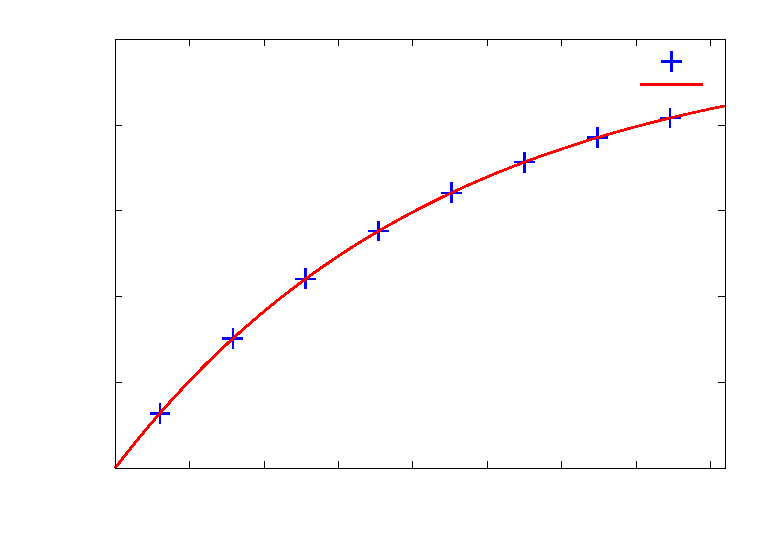
\includegraphics{plots/T1Wasser}}%
    \gplfronttext
  \end{picture}%
\endgroup
}
        \caption{$T_1$-Messung von Wasser.}
        \label{fig:T1Wasser}
    \end{subfigure}
    \begin{subfigure}[b]{0.5\textwidth}
        \centering
        \resizebox{1\textwidth}{!}{% GNUPLOT: LaTeX picture with Postscript
\begingroup
  % Encoding inside the plot.  In the header of your document, this encoding
  % should to defined, e.g., by using
  % \usepackage[cp1252,<other encodings>]{inputenc}
  \inputencoding{cp1252}%
  \makeatletter
  \providecommand\color[2][]{%
    \GenericError{(gnuplot) \space\space\space\@spaces}{%
      Package color not loaded in conjunction with
      terminal option `colourtext'%
    }{See the gnuplot documentation for explanation.%
    }{Either use 'blacktext' in gnuplot or load the package
      color.sty in LaTeX.}%
    \renewcommand\color[2][]{}%
  }%
  \providecommand\includegraphics[2][]{%
    \GenericError{(gnuplot) \space\space\space\@spaces}{%
      Package graphicx or graphics not loaded%
    }{See the gnuplot documentation for explanation.%
    }{The gnuplot epslatex terminal needs graphicx.sty or graphics.sty.}%
    \renewcommand\includegraphics[2][]{}%
  }%
  \providecommand\rotatebox[2]{#2}%
  \@ifundefined{ifGPcolor}{%
    \newif\ifGPcolor
    \GPcolorfalse
  }{}%
  \@ifundefined{ifGPblacktext}{%
    \newif\ifGPblacktext
    \GPblacktexttrue
  }{}%
  % define a \g@addto@macro without @ in the name:
  \let\gplgaddtomacro\g@addto@macro
  % define empty templates for all commands taking text:
  \gdef\gplbacktext{}%
  \gdef\gplfronttext{}%
  \makeatother
  \ifGPblacktext
    % no textcolor at all
    \def\colorrgb#1{}%
    \def\colorgray#1{}%
  \else
    % gray or color?
    \ifGPcolor
      \def\colorrgb#1{\color[rgb]{#1}}%
      \def\colorgray#1{\color[gray]{#1}}%
      \expandafter\def\csname LTw\endcsname{\color{white}}%
      \expandafter\def\csname LTb\endcsname{\color{black}}%
      \expandafter\def\csname LTa\endcsname{\color{black}}%
      \expandafter\def\csname LT0\endcsname{\color[rgb]{1,0,0}}%
      \expandafter\def\csname LT1\endcsname{\color[rgb]{0,1,0}}%
      \expandafter\def\csname LT2\endcsname{\color[rgb]{0,0,1}}%
      \expandafter\def\csname LT3\endcsname{\color[rgb]{1,0,1}}%
      \expandafter\def\csname LT4\endcsname{\color[rgb]{0,1,1}}%
      \expandafter\def\csname LT5\endcsname{\color[rgb]{1,1,0}}%
      \expandafter\def\csname LT6\endcsname{\color[rgb]{0,0,0}}%
      \expandafter\def\csname LT7\endcsname{\color[rgb]{1,0.3,0}}%
      \expandafter\def\csname LT8\endcsname{\color[rgb]{0.5,0.5,0.5}}%
    \else
      % gray
      \def\colorrgb#1{\color{black}}%
      \def\colorgray#1{\color[gray]{#1}}%
      \expandafter\def\csname LTw\endcsname{\color{white}}%
      \expandafter\def\csname LTb\endcsname{\color{black}}%
      \expandafter\def\csname LTa\endcsname{\color{black}}%
      \expandafter\def\csname LT0\endcsname{\color{black}}%
      \expandafter\def\csname LT1\endcsname{\color{black}}%
      \expandafter\def\csname LT2\endcsname{\color{black}}%
      \expandafter\def\csname LT3\endcsname{\color{black}}%
      \expandafter\def\csname LT4\endcsname{\color{black}}%
      \expandafter\def\csname LT5\endcsname{\color{black}}%
      \expandafter\def\csname LT6\endcsname{\color{black}}%
      \expandafter\def\csname LT7\endcsname{\color{black}}%
      \expandafter\def\csname LT8\endcsname{\color{black}}%
    \fi
  \fi
    \setlength{\unitlength}{0.0500bp}%
    \ifx\gptboxheight\undefined%
      \newlength{\gptboxheight}%
      \newlength{\gptboxwidth}%
      \newsavebox{\gptboxtext}%
    \fi%
    \setlength{\fboxrule}{0.5pt}%
    \setlength{\fboxsep}{1pt}%
\begin{picture}(7200.00,5040.00)%
    \gplgaddtomacro\gplbacktext{%
      \csname LTb\endcsname%%
      \put(814,704){\makebox(0,0)[r]{\strut{}$0$}}%
      \put(814,1527){\makebox(0,0)[r]{\strut{}$0.2$}}%
      \put(814,2350){\makebox(0,0)[r]{\strut{}$0.4$}}%
      \put(814,3173){\makebox(0,0)[r]{\strut{}$0.6$}}%
      \put(814,3996){\makebox(0,0)[r]{\strut{}$0.8$}}%
      \put(814,4819){\makebox(0,0)[r]{\strut{}$1$}}%
      \put(946,484){\makebox(0,0){\strut{}$0$}}%
      \put(1922,484){\makebox(0,0){\strut{}$1000$}}%
      \put(2898,484){\makebox(0,0){\strut{}$2000$}}%
      \put(3875,484){\makebox(0,0){\strut{}$3000$}}%
      \put(4851,484){\makebox(0,0){\strut{}$4000$}}%
      \put(5827,484){\makebox(0,0){\strut{}$5000$}}%
      \put(6803,484){\makebox(0,0){\strut{}$6000$}}%
    }%
    \gplgaddtomacro\gplfronttext{%
      \csname LTb\endcsname%%
      \put(308,2761){\rotatebox{-270}{\makebox(0,0){\strut{}Dämpfung $\frac{\text{E}}{\text{E}_0}$}}}%
      \put(3874,154){\makebox(0,0){\strut{}Zeit in $\si{\milli \second}$}}%
      \csname LTb\endcsname%%
      \put(5860,4606){\makebox(0,0)[r]{\strut{}gemessene Datenpunkte für Wasser}}%
      \csname LTb\endcsname%%
      \put(5860,4386){\makebox(0,0)[r]{\strut{}Dämpfungsfit Fit}}%
    }%
    \gplbacktext
    \put(0,0){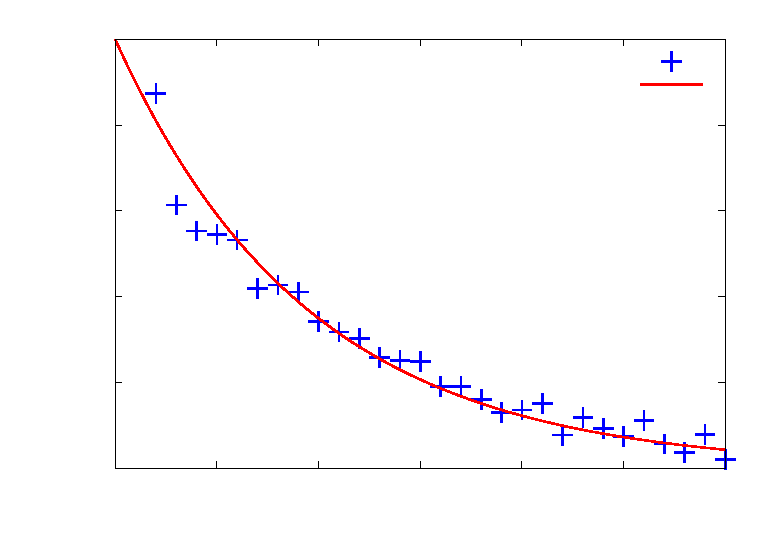
\includegraphics{plots/T2Wasser}}%
    \gplfronttext
  \end{picture}%
\endgroup
}
        \caption{$T_2$-Messung von Wasser.}
        \label{fig:T2Wasser}
    \end{subfigure}
    \caption[$T_1$- und $T_2$-Messung von Wasser.]{Darstellung der typischen Kurvenverläufe bei $T_1$- und $T_2$-Messungen.
    Hierbei konnte, wie in den Abschnitten \ref{sec:LongitudinalrelaxationmeasurementsT1} und \ref{sec:Transversalrelaxationmeasurements} erläutert, jeweils die entsprechende Relaxationszeit $T_1 \approx \SI{2.2}{\second}$ und $T_2 \approx \SI{1.9}{\second}$ ermittelt werden.}
    \label{fig:T1T2Wasser}
\end{figure}

Somit konnte an die Messdaten die jeweilige Formel (\eqref{eq: fitBp} und \eqref{eq:T2}) angefittet werden und $T_1 \approx \SI{2.2}{\second}$ und $T_2 \approx \SI{1.9}{\second}$ als Fitparameter gewonnen werden.
Da als einzige Unsicherheit eine von \textit{GnuPlot} ermittelte mittlere Abweichung berechnet wurde, welche gegenüber der Genauigkeit der Messwerte überaus gering erscheint, wurde hier auf die Angabe derer verzichtet.
Daher wurde auch kein Gleichheitszeichen verwendet. 
Dies könnte vor allem bei $T_1$ darauf zurückzuführen sein, dass die Modelgleichung sehr gut dem Verlauf der Daten entspricht.
Eine entsprechende Übersicht findet sich zudem im Anhang in Tabelle \ref{tab:T1T2}.

Anschließend wurden am Versuchstag acht unterschiedliche Wasserproben in den Aufbau eingesetzt welche jeweils \SI{500}{\milli \liter} Wasser und die oben genannten Stoffmengen an gelöstem Kupfer- oder Mangansalz enthalten.
Für jede dieser Konfigurationen wurde dann eine $T_1$- und eine $T_2$-Messung durchgeführt.
Die gewonnenen Messdaten wurden auf identische Art und Weise wie eben beschrieben analysiert.
Entsprechend finden sich alle Werte für $T_1$ und $T_2$ ebenfalls in Tabelle \ref{tab:T1T2} im Anhang.
Abbildung \ref{fig:T1CU} zeigt beispielhaft alle $T_1$-Messungen mit den unterschiedlichen Konzentrationen des paramagnetischen Kupfers.
Zudem ist zu Referenzzwecken auch die Messreihe des bidestillierten Wassers aufgeführt.
Da erwartet wird, dass die Relaxationszeiten unter Verwendung des Kontrastmittels kürzer sind als jene bei Wasser waren bei der Verwendung des Kontrastmittels steiler Kurvenverläufe zu erwarten.
Dies zeigt sich deutlich in Abbildung \ref{fig:T1CU}. 

\begin{figure}[H]
    \centering
    % GNUPLOT: LaTeX picture with Postscript
\begingroup
  % Encoding inside the plot.  In the header of your document, this encoding
  % should to defined, e.g., by using
  % \usepackage[cp1252,<other encodings>]{inputenc}
  \inputencoding{cp1252}%
  \makeatletter
  \providecommand\color[2][]{%
    \GenericError{(gnuplot) \space\space\space\@spaces}{%
      Package color not loaded in conjunction with
      terminal option `colourtext'%
    }{See the gnuplot documentation for explanation.%
    }{Either use 'blacktext' in gnuplot or load the package
      color.sty in LaTeX.}%
    \renewcommand\color[2][]{}%
  }%
  \providecommand\includegraphics[2][]{%
    \GenericError{(gnuplot) \space\space\space\@spaces}{%
      Package graphicx or graphics not loaded%
    }{See the gnuplot documentation for explanation.%
    }{The gnuplot epslatex terminal needs graphicx.sty or graphics.sty.}%
    \renewcommand\includegraphics[2][]{}%
  }%
  \providecommand\rotatebox[2]{#2}%
  \@ifundefined{ifGPcolor}{%
    \newif\ifGPcolor
    \GPcolorfalse
  }{}%
  \@ifundefined{ifGPblacktext}{%
    \newif\ifGPblacktext
    \GPblacktexttrue
  }{}%
  % define a \g@addto@macro without @ in the name:
  \let\gplgaddtomacro\g@addto@macro
  % define empty templates for all commands taking text:
  \gdef\gplbacktext{}%
  \gdef\gplfronttext{}%
  \makeatother
  \ifGPblacktext
    % no textcolor at all
    \def\colorrgb#1{}%
    \def\colorgray#1{}%
  \else
    % gray or color?
    \ifGPcolor
      \def\colorrgb#1{\color[rgb]{#1}}%
      \def\colorgray#1{\color[gray]{#1}}%
      \expandafter\def\csname LTw\endcsname{\color{white}}%
      \expandafter\def\csname LTb\endcsname{\color{black}}%
      \expandafter\def\csname LTa\endcsname{\color{black}}%
      \expandafter\def\csname LT0\endcsname{\color[rgb]{1,0,0}}%
      \expandafter\def\csname LT1\endcsname{\color[rgb]{0,1,0}}%
      \expandafter\def\csname LT2\endcsname{\color[rgb]{0,0,1}}%
      \expandafter\def\csname LT3\endcsname{\color[rgb]{1,0,1}}%
      \expandafter\def\csname LT4\endcsname{\color[rgb]{0,1,1}}%
      \expandafter\def\csname LT5\endcsname{\color[rgb]{1,1,0}}%
      \expandafter\def\csname LT6\endcsname{\color[rgb]{0,0,0}}%
      \expandafter\def\csname LT7\endcsname{\color[rgb]{1,0.3,0}}%
      \expandafter\def\csname LT8\endcsname{\color[rgb]{0.5,0.5,0.5}}%
    \else
      % gray
      \def\colorrgb#1{\color{black}}%
      \def\colorgray#1{\color[gray]{#1}}%
      \expandafter\def\csname LTw\endcsname{\color{white}}%
      \expandafter\def\csname LTb\endcsname{\color{black}}%
      \expandafter\def\csname LTa\endcsname{\color{black}}%
      \expandafter\def\csname LT0\endcsname{\color{black}}%
      \expandafter\def\csname LT1\endcsname{\color{black}}%
      \expandafter\def\csname LT2\endcsname{\color{black}}%
      \expandafter\def\csname LT3\endcsname{\color{black}}%
      \expandafter\def\csname LT4\endcsname{\color{black}}%
      \expandafter\def\csname LT5\endcsname{\color{black}}%
      \expandafter\def\csname LT6\endcsname{\color{black}}%
      \expandafter\def\csname LT7\endcsname{\color{black}}%
      \expandafter\def\csname LT8\endcsname{\color{black}}%
    \fi
  \fi
    \setlength{\unitlength}{0.0500bp}%
    \ifx\gptboxheight\undefined%
      \newlength{\gptboxheight}%
      \newlength{\gptboxwidth}%
      \newsavebox{\gptboxtext}%
    \fi%
    \setlength{\fboxrule}{0.5pt}%
    \setlength{\fboxsep}{1pt}%
\begin{picture}(7200.00,5040.00)%
    \gplgaddtomacro\gplbacktext{%
      \csname LTb\endcsname%%
      \put(814,704){\makebox(0,0)[r]{\strut{}$0$}}%
      \put(814,1527){\makebox(0,0)[r]{\strut{}$0.2$}}%
      \put(814,2350){\makebox(0,0)[r]{\strut{}$0.4$}}%
      \put(814,3173){\makebox(0,0)[r]{\strut{}$0.6$}}%
      \put(814,3996){\makebox(0,0)[r]{\strut{}$0.8$}}%
      \put(814,4819){\makebox(0,0)[r]{\strut{}$1$}}%
      \put(946,484){\makebox(0,0){\strut{}$0$}}%
      \put(1922,484){\makebox(0,0){\strut{}$1000$}}%
      \put(2898,484){\makebox(0,0){\strut{}$2000$}}%
      \put(3875,484){\makebox(0,0){\strut{}$3000$}}%
      \put(4851,484){\makebox(0,0){\strut{}$4000$}}%
      \put(5827,484){\makebox(0,0){\strut{}$5000$}}%
      \put(6803,484){\makebox(0,0){\strut{}$6000$}}%
    }%
    \gplgaddtomacro\gplfronttext{%
      \csname LTb\endcsname%%
      \put(308,2761){\rotatebox{-270}{\makebox(0,0){\strut{}Dämpfung $\frac{\text{E}}{\text{E}_0}$}}}%
      \put(3874,154){\makebox(0,0){\strut{}Zeit in $\si{\milli \second}$}}%
      \csname LTb\endcsname%%
      \put(5889,3886){\makebox(0,0)[r]{\strut{}$Cu^{2+} \SI{250}{\micro\mole}$}}%
      \csname LTb\endcsname%%
      \put(5889,3666){\makebox(0,0)[r]{\strut{}$Cu^{2+} \SI{500}{\micro\mole}$}}%
      \csname LTb\endcsname%%
      \put(5889,3446){\makebox(0,0)[r]{\strut{}$Cu^{2+} \SI{1000}{\micro\mole}$}}%
      \csname LTb\endcsname%%
      \put(5889,3226){\makebox(0,0)[r]{\strut{}$Cu^{2+} \SI{2000}{\micro\mole}$}}%
      \csname LTb\endcsname%%
      \put(5889,3006){\makebox(0,0)[r]{\strut{}Wasser}}%
    }%
    \gplbacktext
    \put(0,0){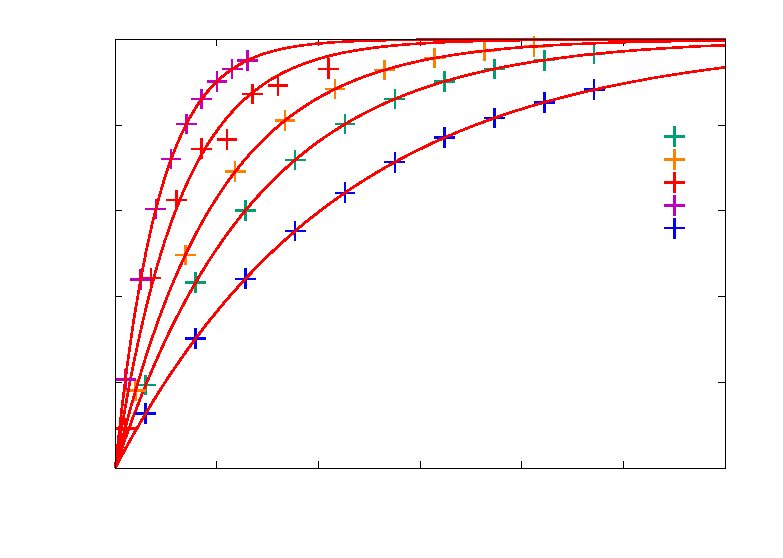
\includegraphics{plots/KupferalleT1}}%
    \gplfronttext
  \end{picture}%
\endgroup

    \caption[Übersicht über alle Messreihen der mit Kupfersalz versetzten Wasserproben.]{Die Abbildung zeigt alle gewonnenen Messreihen der mit unterschiedlichen Konzentrationen von Kupfersalz versetzten Wasserproben.
    Es sind zudem jeweils die nach Formel \eqref{eq: fitBp} durchgeführten Fits zu erkennen.
    Blau ist als Referenz die Messung von bidestilliertem Wasser abgebildet.
    Durch die Farbkodierung ist gut zu erkennen, dass mit zunehmender Konzentration die Kurven steiler verlaufen.
    Dies ist direkt mit kürzeren Relaxationszeiten in Verbindung zu bringen.}
    \label{fig:T1CU}
\end{figure}

Es lässt sich gut erkennen, dass mit zunehmender Kontrastmittelkonzentration ein steilerer Kurvenverlauf vorliegt, was das Abnehmen der longitudinalen Relaxationszeit veranschaulicht.
Ensprechende Abbildungen für $T_2$ und die Messreihen für Mangan finden sich in den Abbildungen \ref{fig:T2CU} bis \ref{fig:T2Mn} im Anhang.

Um die Messungen von Kupfer und Mangan zu vergleichen sind jeweils die Messreihen mit der höchsten und niedrigsten Konzentration des jeweiligen Stoffs sowie Wasser als Referenz in Abbildung \ref{fig:T1CuMn} dargestellt. 

\begin{figure}[H]
    \centering
    % GNUPLOT: LaTeX picture with Postscript
\begingroup
  % Encoding inside the plot.  In the header of your document, this encoding
  % should to defined, e.g., by using
  % \usepackage[cp1252,<other encodings>]{inputenc}
  \inputencoding{cp1252}%
  \makeatletter
  \providecommand\color[2][]{%
    \GenericError{(gnuplot) \space\space\space\@spaces}{%
      Package color not loaded in conjunction with
      terminal option `colourtext'%
    }{See the gnuplot documentation for explanation.%
    }{Either use 'blacktext' in gnuplot or load the package
      color.sty in LaTeX.}%
    \renewcommand\color[2][]{}%
  }%
  \providecommand\includegraphics[2][]{%
    \GenericError{(gnuplot) \space\space\space\@spaces}{%
      Package graphicx or graphics not loaded%
    }{See the gnuplot documentation for explanation.%
    }{The gnuplot epslatex terminal needs graphicx.sty or graphics.sty.}%
    \renewcommand\includegraphics[2][]{}%
  }%
  \providecommand\rotatebox[2]{#2}%
  \@ifundefined{ifGPcolor}{%
    \newif\ifGPcolor
    \GPcolorfalse
  }{}%
  \@ifundefined{ifGPblacktext}{%
    \newif\ifGPblacktext
    \GPblacktexttrue
  }{}%
  % define a \g@addto@macro without @ in the name:
  \let\gplgaddtomacro\g@addto@macro
  % define empty templates for all commands taking text:
  \gdef\gplbacktext{}%
  \gdef\gplfronttext{}%
  \makeatother
  \ifGPblacktext
    % no textcolor at all
    \def\colorrgb#1{}%
    \def\colorgray#1{}%
  \else
    % gray or color?
    \ifGPcolor
      \def\colorrgb#1{\color[rgb]{#1}}%
      \def\colorgray#1{\color[gray]{#1}}%
      \expandafter\def\csname LTw\endcsname{\color{white}}%
      \expandafter\def\csname LTb\endcsname{\color{black}}%
      \expandafter\def\csname LTa\endcsname{\color{black}}%
      \expandafter\def\csname LT0\endcsname{\color[rgb]{1,0,0}}%
      \expandafter\def\csname LT1\endcsname{\color[rgb]{0,1,0}}%
      \expandafter\def\csname LT2\endcsname{\color[rgb]{0,0,1}}%
      \expandafter\def\csname LT3\endcsname{\color[rgb]{1,0,1}}%
      \expandafter\def\csname LT4\endcsname{\color[rgb]{0,1,1}}%
      \expandafter\def\csname LT5\endcsname{\color[rgb]{1,1,0}}%
      \expandafter\def\csname LT6\endcsname{\color[rgb]{0,0,0}}%
      \expandafter\def\csname LT7\endcsname{\color[rgb]{1,0.3,0}}%
      \expandafter\def\csname LT8\endcsname{\color[rgb]{0.5,0.5,0.5}}%
    \else
      % gray
      \def\colorrgb#1{\color{black}}%
      \def\colorgray#1{\color[gray]{#1}}%
      \expandafter\def\csname LTw\endcsname{\color{white}}%
      \expandafter\def\csname LTb\endcsname{\color{black}}%
      \expandafter\def\csname LTa\endcsname{\color{black}}%
      \expandafter\def\csname LT0\endcsname{\color{black}}%
      \expandafter\def\csname LT1\endcsname{\color{black}}%
      \expandafter\def\csname LT2\endcsname{\color{black}}%
      \expandafter\def\csname LT3\endcsname{\color{black}}%
      \expandafter\def\csname LT4\endcsname{\color{black}}%
      \expandafter\def\csname LT5\endcsname{\color{black}}%
      \expandafter\def\csname LT6\endcsname{\color{black}}%
      \expandafter\def\csname LT7\endcsname{\color{black}}%
      \expandafter\def\csname LT8\endcsname{\color{black}}%
    \fi
  \fi
    \setlength{\unitlength}{0.0500bp}%
    \ifx\gptboxheight\undefined%
      \newlength{\gptboxheight}%
      \newlength{\gptboxwidth}%
      \newsavebox{\gptboxtext}%
    \fi%
    \setlength{\fboxrule}{0.5pt}%
    \setlength{\fboxsep}{1pt}%
\begin{picture}(7200.00,5040.00)%
    \gplgaddtomacro\gplbacktext{%
      \csname LTb\endcsname%%
      \put(814,704){\makebox(0,0)[r]{\strut{}$0$}}%
      \put(814,1527){\makebox(0,0)[r]{\strut{}$0.2$}}%
      \put(814,2350){\makebox(0,0)[r]{\strut{}$0.4$}}%
      \put(814,3173){\makebox(0,0)[r]{\strut{}$0.6$}}%
      \put(814,3996){\makebox(0,0)[r]{\strut{}$0.8$}}%
      \put(814,4819){\makebox(0,0)[r]{\strut{}$1$}}%
      \put(946,484){\makebox(0,0){\strut{}$0$}}%
      \put(1922,484){\makebox(0,0){\strut{}$1000$}}%
      \put(2898,484){\makebox(0,0){\strut{}$2000$}}%
      \put(3875,484){\makebox(0,0){\strut{}$3000$}}%
      \put(4851,484){\makebox(0,0){\strut{}$4000$}}%
      \put(5827,484){\makebox(0,0){\strut{}$5000$}}%
      \put(6803,484){\makebox(0,0){\strut{}$6000$}}%
    }%
    \gplgaddtomacro\gplfronttext{%
      \csname LTb\endcsname%%
      \put(308,2761){\rotatebox{-270}{\makebox(0,0){\strut{}D\"ampfung $\frac{\text{E}}{\text{E}_0}$}}}%
      \put(3874,154){\makebox(0,0){\strut{}Zeit in $\si{\milli \second}$}}%
      \csname LTb\endcsname%%
      \put(5860,3680){\makebox(0,0)[r]{\strut{}Wasser}}%
      \csname LTb\endcsname%%
      \put(5860,3460){\makebox(0,0)[r]{\strut{}$Cu^{2+}$ $\SI{250}{\micro\mole}$}}%
      \csname LTb\endcsname%%
      \put(5860,3240){\makebox(0,0)[r]{\strut{}$Mn^{2+}$ $\SI{25}{\micro\mole}$}}%
      \csname LTb\endcsname%%
      \put(5860,3020){\makebox(0,0)[r]{\strut{}$Cu^{2+}$ $\SI{2000}{\micro\mole}$}}%
      \csname LTb\endcsname%%
      \put(5860,2800){\makebox(0,0)[r]{\strut{}$Mn^{2+}$ $\SI{200}{\micro\mole}$}}%
    }%
    \gplbacktext
    \put(0,0){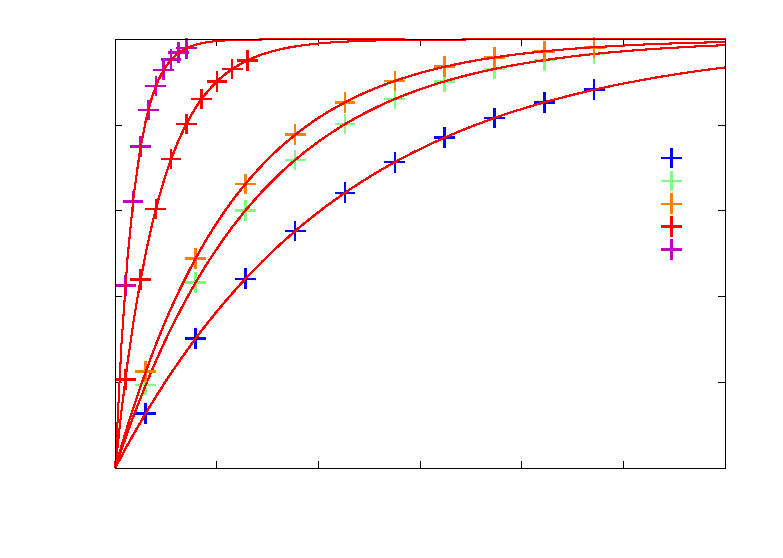
\includegraphics{plots/CuMnVgl}}%
    \gplfronttext
  \end{picture}%
\endgroup

    \caption[Vergleichende Darstellung der $T_1$-Messreihen kupfer- und manganversetzter Wasserproben.]{Vergleichende Darstellung der $T_1$-Messreihen kupfer- und manganversetzter Wasserproben. Dabei ist zu erkennen, dass bereits ein Zehntel der Stoffmenge von Mangan ähnliche Resultat hervorbringt wie die an Kupfer verwendete Stoffmenge.}
    \label{fig:T1CuMn}
\end{figure}

Es zeigt sich, dass beide Stoffe in den ,,extremen'' Konzentrationen ähnlich starke Auswirkungen auf die Relaxationszeit aufweisen.
Dabei ist allerdings festzuhalten, dass von Mangan nur ein Zehntel der Stoffmenge für einen ähnlichen Effekt von Nöten ist.
Da, wie oben erwähnt, geringe Kontrastmittelkonzentration sich besonders gut für die Manipulation der longitudinalen Relaxationszeit eignen und hohe Konzentrationen besser für die transversale Relaxationszeit geeignet sind, lässt sich folgern, dass mittels Kupfersalz $T_1$-Messungen besser kontrolliert werden können.
Dies ist dadurch zu begründen, dass recht hohe Stoffmengen benötigt werden und somit genauer dosiert werden kann.
Mangan hingegen könnte sich besser für $T_2$-Effekte eignen, da bereits vergleichsweise geringe Stoffmengen großen Einfluss nehmen und somit bei groß gewählter Stoffmenge die Messunge deutlich an Intensität verlieren.

Um diese Vermutung weiter zu quantifizieren konnten die Relaxivitäten $r_1$ und $r_2$ nach Formel \eqref{eq:relaxivitat}von Kupfer und Mangan berechnet werden.
Dazu wurden die verwendeten Stoffmengen in Konzentrationen umgerechnet und die Kehrwerte der in Tabelle \ref{tab:T1T2} aufgeführten Relaxationszeiten jeweils über diesen Konzentrationen aufgetragen.

\begin{figure}[H]
    \centering
    % GNUPLOT: LaTeX picture with Postscript
\begingroup
  % Encoding inside the plot.  In the header of your document, this encoding
  % should to defined, e.g., by using
  % \usepackage[cp1252,<other encodings>]{inputenc}
  \inputencoding{cp1252}%
  \makeatletter
  \providecommand\color[2][]{%
    \GenericError{(gnuplot) \space\space\space\@spaces}{%
      Package color not loaded in conjunction with
      terminal option `colourtext'%
    }{See the gnuplot documentation for explanation.%
    }{Either use 'blacktext' in gnuplot or load the package
      color.sty in LaTeX.}%
    \renewcommand\color[2][]{}%
  }%
  \providecommand\includegraphics[2][]{%
    \GenericError{(gnuplot) \space\space\space\@spaces}{%
      Package graphicx or graphics not loaded%
    }{See the gnuplot documentation for explanation.%
    }{The gnuplot epslatex terminal needs graphicx.sty or graphics.sty.}%
    \renewcommand\includegraphics[2][]{}%
  }%
  \providecommand\rotatebox[2]{#2}%
  \@ifundefined{ifGPcolor}{%
    \newif\ifGPcolor
    \GPcolorfalse
  }{}%
  \@ifundefined{ifGPblacktext}{%
    \newif\ifGPblacktext
    \GPblacktexttrue
  }{}%
  % define a \g@addto@macro without @ in the name:
  \let\gplgaddtomacro\g@addto@macro
  % define empty templates for all commands taking text:
  \gdef\gplbacktext{}%
  \gdef\gplfronttext{}%
  \makeatother
  \ifGPblacktext
    % no textcolor at all
    \def\colorrgb#1{}%
    \def\colorgray#1{}%
  \else
    % gray or color?
    \ifGPcolor
      \def\colorrgb#1{\color[rgb]{#1}}%
      \def\colorgray#1{\color[gray]{#1}}%
      \expandafter\def\csname LTw\endcsname{\color{white}}%
      \expandafter\def\csname LTb\endcsname{\color{black}}%
      \expandafter\def\csname LTa\endcsname{\color{black}}%
      \expandafter\def\csname LT0\endcsname{\color[rgb]{1,0,0}}%
      \expandafter\def\csname LT1\endcsname{\color[rgb]{0,1,0}}%
      \expandafter\def\csname LT2\endcsname{\color[rgb]{0,0,1}}%
      \expandafter\def\csname LT3\endcsname{\color[rgb]{1,0,1}}%
      \expandafter\def\csname LT4\endcsname{\color[rgb]{0,1,1}}%
      \expandafter\def\csname LT5\endcsname{\color[rgb]{1,1,0}}%
      \expandafter\def\csname LT6\endcsname{\color[rgb]{0,0,0}}%
      \expandafter\def\csname LT7\endcsname{\color[rgb]{1,0.3,0}}%
      \expandafter\def\csname LT8\endcsname{\color[rgb]{0.5,0.5,0.5}}%
    \else
      % gray
      \def\colorrgb#1{\color{black}}%
      \def\colorgray#1{\color[gray]{#1}}%
      \expandafter\def\csname LTw\endcsname{\color{white}}%
      \expandafter\def\csname LTb\endcsname{\color{black}}%
      \expandafter\def\csname LTa\endcsname{\color{black}}%
      \expandafter\def\csname LT0\endcsname{\color{black}}%
      \expandafter\def\csname LT1\endcsname{\color{black}}%
      \expandafter\def\csname LT2\endcsname{\color{black}}%
      \expandafter\def\csname LT3\endcsname{\color{black}}%
      \expandafter\def\csname LT4\endcsname{\color{black}}%
      \expandafter\def\csname LT5\endcsname{\color{black}}%
      \expandafter\def\csname LT6\endcsname{\color{black}}%
      \expandafter\def\csname LT7\endcsname{\color{black}}%
      \expandafter\def\csname LT8\endcsname{\color{black}}%
    \fi
  \fi
    \setlength{\unitlength}{0.0500bp}%
    \ifx\gptboxheight\undefined%
      \newlength{\gptboxheight}%
      \newlength{\gptboxwidth}%
      \newsavebox{\gptboxtext}%
    \fi%
    \setlength{\fboxrule}{0.5pt}%
    \setlength{\fboxsep}{1pt}%
\begin{picture}(7200.00,5040.00)%
    \gplgaddtomacro\gplbacktext{%
      \csname LTb\endcsname%%
      \put(1474,704){\makebox(0,0)[r]{\strut{}$0.0*10^{0}$}}%
      \put(1474,1292){\makebox(0,0)[r]{\strut{}$5.0*10^{-4}$}}%
      \put(1474,1880){\makebox(0,0)[r]{\strut{}$1.0*10^{-3}$}}%
      \put(1474,2468){\makebox(0,0)[r]{\strut{}$1.5*10^{-3}$}}%
      \put(1474,3055){\makebox(0,0)[r]{\strut{}$2.0*10^{-3}$}}%
      \put(1474,3643){\makebox(0,0)[r]{\strut{}$2.5*10^{-3}$}}%
      \put(1474,4231){\makebox(0,0)[r]{\strut{}$3.0*10^{-3}$}}%
      \put(1474,4819){\makebox(0,0)[r]{\strut{}$3.5*10^{-3}$}}%
      \put(1606,484){\makebox(0,0){\strut{}$0$}}%
      \put(2645,484){\makebox(0,0){\strut{}$1$}}%
      \put(3685,484){\makebox(0,0){\strut{}$2$}}%
      \put(4724,484){\makebox(0,0){\strut{}$3$}}%
      \put(5764,484){\makebox(0,0){\strut{}$4$}}%
      \put(6803,484){\makebox(0,0){\strut{}$5$}}%
    }%
    \gplgaddtomacro\gplfronttext{%
      \csname LTb\endcsname%%
      \put(308,2761){\rotatebox{-270}{\makebox(0,0){\strut{}Kehrwert der Zeit in $\si{\per \second}$}}}%
      \put(4204,154){\makebox(0,0){\strut{}Konzentration in  $\si{\mol \per \meter \tothe{3} }$}}%
      \csname LTb\endcsname%%
      \put(5870,4606){\makebox(0,0)[r]{\strut{}$1/T_{\text{1}}\left([\ce{Cu^2+}]\right)$}}%
      \csname LTb\endcsname%%
      \put(5870,4386){\makebox(0,0)[r]{\strut{}linearer Fit}}%
    }%
    \gplbacktext
    \put(0,0){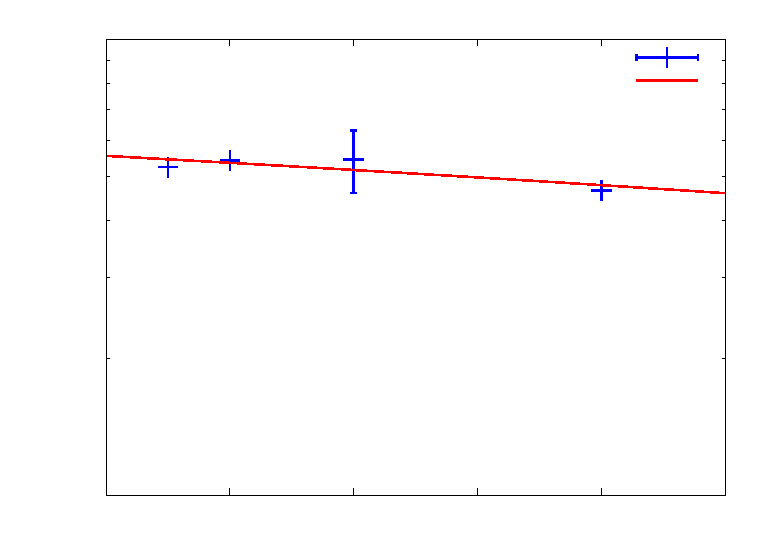
\includegraphics{plots/Relaxivitat_CuT1}}%
    \gplfronttext
  \end{picture}%
\endgroup

    \caption[Linearer Fit zur Ermittlung der Relaxivität $r_1$ von Kupfer.]{Diese Abbildung zeigt die Kehrwerte der vier Relaxationszeiten $T_1$ aufgetragen über den entsprechenden Konzentrationen des im Wasser gelösten Kupfersalzes. Mittels eines linearen Fits konnten somit die Relaxivität $r_1$ -- als Steigung -- sowie die Relaxationszeit ohne gelöstes Kontrastmittel nach Gleichung \eqref{eq:relaxivitat} ermittlet werden.}
    \label{fig:RelaxCUT1}
\end{figure}

Beispielhaft zeigt Abbildung \ref{fig:RelaxCUT1} eine solche Darstellung.
Alle weiteren Graphen sind im Anhang in Abbildung \ref{fig:RelaxAlle} zu finden.
Mittels linearem Fit konnte dann entsprechend die Relaxivität, sowie zu Kontrollzwecken der Kehrwert der jeweiligen Relaxationszeit ermittelt werden.
Letzterer ergibt sich als y-Achsenabschnitt, die Relaxivität hingegen ist durch die Steigung des Graphen gegeben.
Eine hohe Relaxivität ist somit ein Indikator dafür, dass schon geringe Stoffmengen die Relaxationszeiten deutlich verringern.
Eine Übersicht über alle gewonnenen Daten findet sich in Tabelle \ref{tab:Relaxivitat}.

\begin{table}[H]
    \centering
    \caption{Relaxivitäten von Kupfer und Mangan.}
    \begin{tabular}{|l||r|r|r|r|} \hline
        Kontrastmittel & $r_{1}$ in $\si{\frac{\mol}{\metre \cubed \second}}$    &  $T_{1}(0)$ in $\si{\second}$ & $r_{2}$ in $\si{\frac{\mol}{\metre \cubed \second}}$ & $T_{2}(0)$ in $\si{\second}$  \\ \hline \hline
        Kupfer & $\SI{0.454 \pm 0.031}{}$   & $\SI{1.84 \pm 0.24}{}$    & $\SI{0.617 \pm 0.084}{}$   & $\SI{2.9  \pm 1.6}{}$ \\ \hline
        Mangan & $\SI{13.65 \pm 0.84}{}$    & $\SI{5.7 \pm 6.3}{}$      & $\SI{35.9 \pm 3.1}{}$  & $\SI{-3.2 \pm 7.5}{}$ \\ \hline
    \end{tabular} 
    \label{tab:Relaxivitat} 
\end{table}

Da die Relaxivitäten ein Maß für die Abnahme der Relaxationszeiten pro Stoffkonzentration sind, geben diese Aufschluss darüber, welcher Stoff sich wie stark auf $T_1$ und $T_2$ auswirkt und ob es gegebenenfalls Unterschiede in der Wirksamkeit bei $T_1$ und $T_2$ gibt.
Aus Tabelle \ref{tab:Relaxivitat} ist zu erkennen, dass sich die Relaxivitäten $r_1$ und $r_2$ von Kupfer kaum unterscheiden.
Jene von Mangan hingegen deutlich.
Dies unterstreicht die vorhergegangen Vermutung, dass sich Mangan als Kontrastmittel zur Beeinflussung der transversalen Relaxationszeiten deutlich besser eignet als Kupfer.
Unterstützt werden obige Vermutungen zudem dadurch, dass die Werte von Mangan mehr als eine Größenordnung größer sind als die von Kupfer.
Dies bedeutet, dass bereits eine geringe Stoffmenge Mangan ausreicht um die Relaxivität deutlich zu steigerm.
Die aufgeführten Relaxationszeiten sollen hier als Referenzgröße zur Überprüfung der Genauigkeit der erhaltenen Werte dienen.
Die Ursprünglich für Wasser gewonnen Relaxationszeiten lagen bei ca. \SI{2}{\second}.
Entsprechend liegen zumindest die Werte für Kupfer im Rahmen der angegebenen Unsicherheiten in der gleichen Größenordnung.
Dies unterstreicht die Validität der ermittelten Relaxivitäten.
Bei Mangan trifft dies zwar auch zu, allerdings liegen sowohl die Werte von $T_1(0)$ und $T_2(0)$ wie auch deren Unsicherheiten bei deutlich höheren Werten und sind somit nur aufgrund der großen Unsicherheiten mit den vorab bestimmten Werten vereinbar.
Auffällig ist ebenfalls, dass $T_{2,\text{Mn}}$ einen negativen Wert aufweist.
Dies ist physikalisch nicht sinnvoll und dadurch zu erklären, dass der Fit nur auf Grundlage von vier Messwerten angefertigt wurde und der Wert aus dem Kehrwert des y-Achsenabschnitts gewonnen wurde.
Entsprechend groß ist auch der Wert der zugehörigen Unsicherheit.
Dadurch kann der negative Wert eingeordnet werden und lässt zudem den Rückschluss zu, dass eine qualitative Betrachtung an dieser Stelle sinnvoller ist und die berechneten Werte eher als ein Maß für die Größenordnung aufgefasst werden sollten.

Die entsprechenden Unsicherheiten wurden den Fits durch \textit{GnuPlot} entnommen und mittels \textsc{Gauss}'scher Fehlerfortpflanzungsformel weitergeführt.
Da der Versuch per Computer durchgeführt wurde, fällt es schwer einzuschätzen, ob sich diese durch eine andere Vorgehensweise am Versuchstag hätten minimieren lassen oder ob es Einflüsse vor Ort gab, welchen hätte entgegengewirkt werden können.
    
    % \begin{figure}[H]
    %     \centering
    %     % GNUPLOT: LaTeX picture with Postscript
\begingroup
  % Encoding inside the plot.  In the header of your document, this encoding
  % should to defined, e.g., by using
  % \usepackage[cp1252,<other encodings>]{inputenc}
  \inputencoding{cp1252}%
  \makeatletter
  \providecommand\color[2][]{%
    \GenericError{(gnuplot) \space\space\space\@spaces}{%
      Package color not loaded in conjunction with
      terminal option `colourtext'%
    }{See the gnuplot documentation for explanation.%
    }{Either use 'blacktext' in gnuplot or load the package
      color.sty in LaTeX.}%
    \renewcommand\color[2][]{}%
  }%
  \providecommand\includegraphics[2][]{%
    \GenericError{(gnuplot) \space\space\space\@spaces}{%
      Package graphicx or graphics not loaded%
    }{See the gnuplot documentation for explanation.%
    }{The gnuplot epslatex terminal needs graphicx.sty or graphics.sty.}%
    \renewcommand\includegraphics[2][]{}%
  }%
  \providecommand\rotatebox[2]{#2}%
  \@ifundefined{ifGPcolor}{%
    \newif\ifGPcolor
    \GPcolorfalse
  }{}%
  \@ifundefined{ifGPblacktext}{%
    \newif\ifGPblacktext
    \GPblacktexttrue
  }{}%
  % define a \g@addto@macro without @ in the name:
  \let\gplgaddtomacro\g@addto@macro
  % define empty templates for all commands taking text:
  \gdef\gplbacktext{}%
  \gdef\gplfronttext{}%
  \makeatother
  \ifGPblacktext
    % no textcolor at all
    \def\colorrgb#1{}%
    \def\colorgray#1{}%
  \else
    % gray or color?
    \ifGPcolor
      \def\colorrgb#1{\color[rgb]{#1}}%
      \def\colorgray#1{\color[gray]{#1}}%
      \expandafter\def\csname LTw\endcsname{\color{white}}%
      \expandafter\def\csname LTb\endcsname{\color{black}}%
      \expandafter\def\csname LTa\endcsname{\color{black}}%
      \expandafter\def\csname LT0\endcsname{\color[rgb]{1,0,0}}%
      \expandafter\def\csname LT1\endcsname{\color[rgb]{0,1,0}}%
      \expandafter\def\csname LT2\endcsname{\color[rgb]{0,0,1}}%
      \expandafter\def\csname LT3\endcsname{\color[rgb]{1,0,1}}%
      \expandafter\def\csname LT4\endcsname{\color[rgb]{0,1,1}}%
      \expandafter\def\csname LT5\endcsname{\color[rgb]{1,1,0}}%
      \expandafter\def\csname LT6\endcsname{\color[rgb]{0,0,0}}%
      \expandafter\def\csname LT7\endcsname{\color[rgb]{1,0.3,0}}%
      \expandafter\def\csname LT8\endcsname{\color[rgb]{0.5,0.5,0.5}}%
    \else
      % gray
      \def\colorrgb#1{\color{black}}%
      \def\colorgray#1{\color[gray]{#1}}%
      \expandafter\def\csname LTw\endcsname{\color{white}}%
      \expandafter\def\csname LTb\endcsname{\color{black}}%
      \expandafter\def\csname LTa\endcsname{\color{black}}%
      \expandafter\def\csname LT0\endcsname{\color{black}}%
      \expandafter\def\csname LT1\endcsname{\color{black}}%
      \expandafter\def\csname LT2\endcsname{\color{black}}%
      \expandafter\def\csname LT3\endcsname{\color{black}}%
      \expandafter\def\csname LT4\endcsname{\color{black}}%
      \expandafter\def\csname LT5\endcsname{\color{black}}%
      \expandafter\def\csname LT6\endcsname{\color{black}}%
      \expandafter\def\csname LT7\endcsname{\color{black}}%
      \expandafter\def\csname LT8\endcsname{\color{black}}%
    \fi
  \fi
    \setlength{\unitlength}{0.0500bp}%
    \ifx\gptboxheight\undefined%
      \newlength{\gptboxheight}%
      \newlength{\gptboxwidth}%
      \newsavebox{\gptboxtext}%
    \fi%
    \setlength{\fboxrule}{0.5pt}%
    \setlength{\fboxsep}{1pt}%
\begin{picture}(7200.00,5040.00)%
    \gplgaddtomacro\gplbacktext{%
      \csname LTb\endcsname%%
      \put(1078,704){\makebox(0,0)[r]{\strut{}$0$}}%
      \put(1078,1161){\makebox(0,0)[r]{\strut{}$2000$}}%
      \put(1078,1618){\makebox(0,0)[r]{\strut{}$4000$}}%
      \put(1078,2076){\makebox(0,0)[r]{\strut{}$6000$}}%
      \put(1078,2533){\makebox(0,0)[r]{\strut{}$8000$}}%
      \put(1078,2990){\makebox(0,0)[r]{\strut{}$10000$}}%
      \put(1078,3447){\makebox(0,0)[r]{\strut{}$12000$}}%
      \put(1078,3905){\makebox(0,0)[r]{\strut{}$14000$}}%
      \put(1078,4362){\makebox(0,0)[r]{\strut{}$16000$}}%
      \put(1078,4819){\makebox(0,0)[r]{\strut{}$18000$}}%
      \put(1210,484){\makebox(0,0){\strut{}$1800$}}%
      \put(2329,484){\makebox(0,0){\strut{}$1820$}}%
      \put(3447,484){\makebox(0,0){\strut{}$1840$}}%
      \put(4566,484){\makebox(0,0){\strut{}$1860$}}%
      \put(5684,484){\makebox(0,0){\strut{}$1880$}}%
      \put(6803,484){\makebox(0,0){\strut{}$1900$}}%
    }%
    \gplgaddtomacro\gplfronttext{%
      \csname LTb\endcsname%%
      \put(198,2761){\rotatebox{-270}{\makebox(0,0){\strut{}Amplitude in willk\"urlicher Enheit}}}%
      \put(4006,154){\makebox(0,0){\strut{}Frequenz in $\si{\hertz}$}}%
      \csname LTb\endcsname%%
      \put(5816,4646){\makebox(0,0)[r]{\strut{}Signal von $Cu^{2+}$ $T_{2}$ mit $\SI{250}{\micro\mole}$}}%
      \csname LTb\endcsname%%
      \put(5816,4426){\makebox(0,0)[r]{\strut{}Signal von $Cu^{2+}$ $T_{2}$ mit $\SI{500}{\micro\mole}$}}%
      \csname LTb\endcsname%%
      \put(5816,4206){\makebox(0,0)[r]{\strut{}Signal von $Cu^{2+}$ $T_{2}$ mit $\SI{1000}{\micro\mole}$}}%
    }%
    \gplbacktext
    \put(0,0){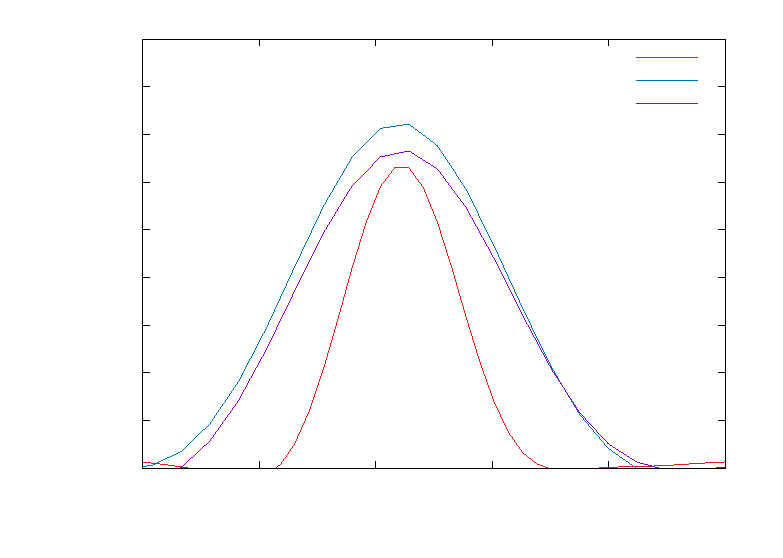
\includegraphics{plots/SignalkontrastT2}}%
    \gplfronttext
  \end{picture}%
\endgroup

    %     \caption{Die T2 Signale bei der jeweiligen Konzentration}
    % \end{figure}
    %  ich glaube die Abbildung ist nicht gut genug, 
    % bzw. die Fehlerdiskussion hätte ich keine Ahnung, warum 1000mol in der Mitte von den zwei ist

% \begin{figure}[H]
%     \centering
%     % GNUPLOT: LaTeX picture with Postscript
\begingroup
  % Encoding inside the plot.  In the header of your document, this encoding
  % should to defined, e.g., by using
  % \usepackage[cp1252,<other encodings>]{inputenc}
  \inputencoding{cp1252}%
  \makeatletter
  \providecommand\color[2][]{%
    \GenericError{(gnuplot) \space\space\space\@spaces}{%
      Package color not loaded in conjunction with
      terminal option `colourtext'%
    }{See the gnuplot documentation for explanation.%
    }{Either use 'blacktext' in gnuplot or load the package
      color.sty in LaTeX.}%
    \renewcommand\color[2][]{}%
  }%
  \providecommand\includegraphics[2][]{%
    \GenericError{(gnuplot) \space\space\space\@spaces}{%
      Package graphicx or graphics not loaded%
    }{See the gnuplot documentation for explanation.%
    }{The gnuplot epslatex terminal needs graphicx.sty or graphics.sty.}%
    \renewcommand\includegraphics[2][]{}%
  }%
  \providecommand\rotatebox[2]{#2}%
  \@ifundefined{ifGPcolor}{%
    \newif\ifGPcolor
    \GPcolorfalse
  }{}%
  \@ifundefined{ifGPblacktext}{%
    \newif\ifGPblacktext
    \GPblacktexttrue
  }{}%
  % define a \g@addto@macro without @ in the name:
  \let\gplgaddtomacro\g@addto@macro
  % define empty templates for all commands taking text:
  \gdef\gplbacktext{}%
  \gdef\gplfronttext{}%
  \makeatother
  \ifGPblacktext
    % no textcolor at all
    \def\colorrgb#1{}%
    \def\colorgray#1{}%
  \else
    % gray or color?
    \ifGPcolor
      \def\colorrgb#1{\color[rgb]{#1}}%
      \def\colorgray#1{\color[gray]{#1}}%
      \expandafter\def\csname LTw\endcsname{\color{white}}%
      \expandafter\def\csname LTb\endcsname{\color{black}}%
      \expandafter\def\csname LTa\endcsname{\color{black}}%
      \expandafter\def\csname LT0\endcsname{\color[rgb]{1,0,0}}%
      \expandafter\def\csname LT1\endcsname{\color[rgb]{0,1,0}}%
      \expandafter\def\csname LT2\endcsname{\color[rgb]{0,0,1}}%
      \expandafter\def\csname LT3\endcsname{\color[rgb]{1,0,1}}%
      \expandafter\def\csname LT4\endcsname{\color[rgb]{0,1,1}}%
      \expandafter\def\csname LT5\endcsname{\color[rgb]{1,1,0}}%
      \expandafter\def\csname LT6\endcsname{\color[rgb]{0,0,0}}%
      \expandafter\def\csname LT7\endcsname{\color[rgb]{1,0.3,0}}%
      \expandafter\def\csname LT8\endcsname{\color[rgb]{0.5,0.5,0.5}}%
    \else
      % gray
      \def\colorrgb#1{\color{black}}%
      \def\colorgray#1{\color[gray]{#1}}%
      \expandafter\def\csname LTw\endcsname{\color{white}}%
      \expandafter\def\csname LTb\endcsname{\color{black}}%
      \expandafter\def\csname LTa\endcsname{\color{black}}%
      \expandafter\def\csname LT0\endcsname{\color{black}}%
      \expandafter\def\csname LT1\endcsname{\color{black}}%
      \expandafter\def\csname LT2\endcsname{\color{black}}%
      \expandafter\def\csname LT3\endcsname{\color{black}}%
      \expandafter\def\csname LT4\endcsname{\color{black}}%
      \expandafter\def\csname LT5\endcsname{\color{black}}%
      \expandafter\def\csname LT6\endcsname{\color{black}}%
      \expandafter\def\csname LT7\endcsname{\color{black}}%
      \expandafter\def\csname LT8\endcsname{\color{black}}%
    \fi
  \fi
    \setlength{\unitlength}{0.0500bp}%
    \ifx\gptboxheight\undefined%
      \newlength{\gptboxheight}%
      \newlength{\gptboxwidth}%
      \newsavebox{\gptboxtext}%
    \fi%
    \setlength{\fboxrule}{0.5pt}%
    \setlength{\fboxsep}{1pt}%
\begin{picture}(7200.00,5040.00)%
    \gplgaddtomacro\gplbacktext{%
      \csname LTb\endcsname%%
      \put(682,704){\makebox(0,0)[r]{\strut{}$0$}}%
      \put(682,1390){\makebox(0,0)[r]{\strut{}$5$}}%
      \put(682,2076){\makebox(0,0)[r]{\strut{}$10$}}%
      \put(682,2762){\makebox(0,0)[r]{\strut{}$15$}}%
      \put(682,3447){\makebox(0,0)[r]{\strut{}$20$}}%
      \put(682,4133){\makebox(0,0)[r]{\strut{}$25$}}%
      \put(682,4819){\makebox(0,0)[r]{\strut{}$30$}}%
      \put(814,484){\makebox(0,0){\strut{}$1800$}}%
      \put(2012,484){\makebox(0,0){\strut{}$1820$}}%
      \put(3210,484){\makebox(0,0){\strut{}$1840$}}%
      \put(4407,484){\makebox(0,0){\strut{}$1860$}}%
      \put(5605,484){\makebox(0,0){\strut{}$1880$}}%
      \put(6803,484){\makebox(0,0){\strut{}$1900$}}%
    }%
    \gplgaddtomacro\gplfronttext{%
      \csname LTb\endcsname%%
      \put(198,2761){\rotatebox{-270}{\makebox(0,0){\strut{}Amplitude in $\si{\frac{\mu \volt}{\hertz}}$}}}%
      \put(3808,154){\makebox(0,0){\strut{}Frequenz in $\si{\hertz}$}}%
      \csname LTb\endcsname%%
      \put(5816,4646){\makebox(0,0)[r]{\strut{}Signal von $Cu^{2+}$ $T_{1}$ mit $\SI{250}{\micro\mole}$}}%
      \csname LTb\endcsname%%
      \put(5816,4426){\makebox(0,0)[r]{\strut{}Signal von $Cu^{2+}$ $T_{1}$ $\SI{500}{\micro\mole}$}}%
    }%
    \gplbacktext
    \put(0,0){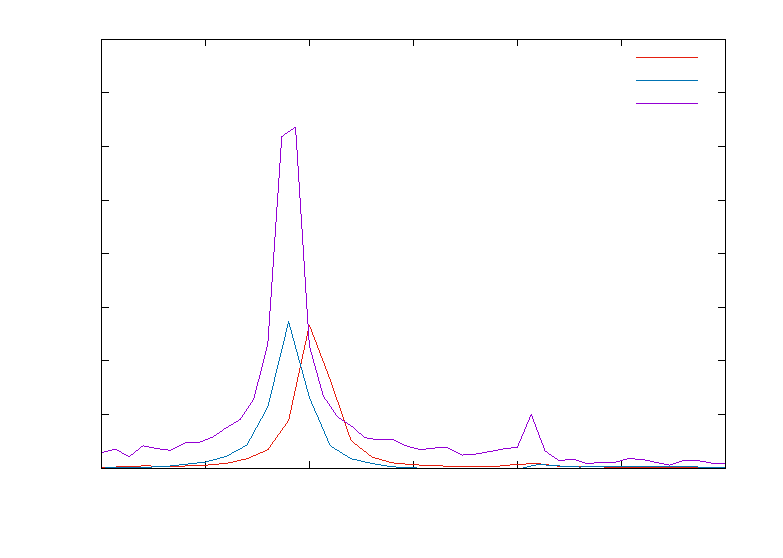
\includegraphics{plots/SignalkontrastT1}}%
    \gplfronttext
  \end{picture}%
\endgroup

%     \caption{Die T1 Signale bei der jeweiligen Konzentration}
%     \label{fig:T1Signalkontrast}
% \end{figure}